\subsubsection{Introduction}

The aim of Part b is to apply ``Dropout'' to the neural network designed in Part
A. The hyperperameters, i.e. the dropout rate, needs to be tuned in order to
obtain an optimal performance from the network.

\subsubsection{Rational}

Dropout is a technique used in Neural Networks in order to prevent over-fitting.
By dropping certain neurons at random during testing, the network must learn
features which are considered ``robust''. This will lead to a greater test
accuracy.

\subsubsection{Design}

Dropout layers are

\subsubsection{Testing}

For the purposes of testing, the dropout rate was the hyperparameter being
tuned. The dropout rate of the first two dropout layers was set to 0.1 as a
baseline measurement, while the rate of the dropout rate before the final
``Dense'' layer was modified. This resulted in an optimum value of 0.5 given for
the final dropout layer, as shown in the table below.

\begin{table}[H]
	\centering
	\caption{Dropout Hyperparameter Tuning}
	\label{tab:d1hyp}
	\begin{tabular}{|c|c|}
	\hline
	Dropout Rate & Validation Accuracy \\
	\hline
	0.55 & 77.83\\
	0.5 & 78.5 \\
	0.25 & 74.7 \\
	0.1 & 76.17 \\
	\hline
	\end{tabular}
\end{table}

Setting this dropout rate, the dropout rates of the other two dropout layers are
changed simultaneously. The optimal value given by the testing was 0.1. This
value is not shown in the table below, as it had previously been tested in the
table above.

\begin{table}[H]
	\centering
	\caption{Dropout Hyperparameter Tuning}
	\label{tab:d2hyp}
	\begin{tabular}{|c|c|}
	\hline
	Dropout Rate & Validation Accuracy \\
	0.55 & 73.83 \\
	0.5 & 77.83\\
	0.25 & 77 \\
	\hline
	\hline
	\end{tabular}
\end{table}

Using this value for the dropout rate, the earling stopping patience value was
increased to 7, and the training was set to run for 30 epochs.

\subsubsection{Results}

The output for the neuran network structure was again printed using the
``model.summary'' function in keras, as seen in Figure \ref{fig:q1pbmodel}.
This shows the placement of the Dropout layers, as previously discussed.

\begin{figure}[H]
	\centering
	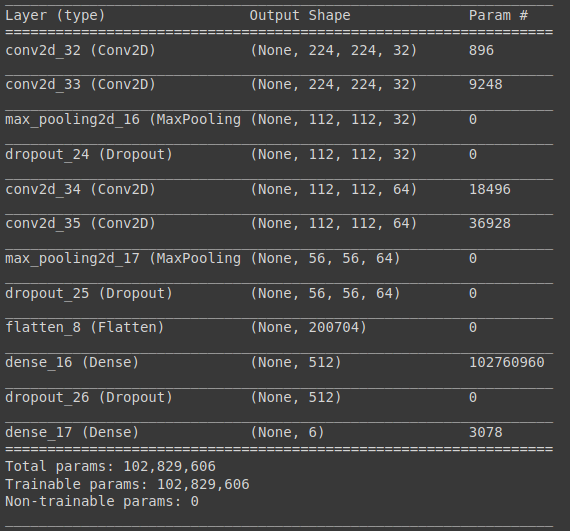
\includegraphics[width=0.8\textwidth]{images/q1/pb/q1pbmodel}
	\caption{Model Summary}
	\label{fig:q1pbmodel}
\end{figure}

Figures \ref{fig:q1pbacc} and \ref{fig:q1pbloss} again show that overfitting is
not occurring. While the accuracy is on an upward trend, it does begin to trail
downwards towards the final epochs.

\begin{figure}[H]
	\centering
	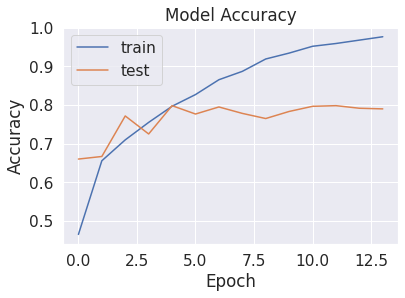
\includegraphics[width=0.8\textwidth]{images/q1/pb/accuracy}
	\caption{Validation and Training Accuracy}
	\label{fig:q1pbacc}
\end{figure}

Again, the loss value is much higher than that of the training, however it is
lower than in Part a, with a value of approximately 1/2 that of Part a.

\begin{figure}[H]
	\centering
	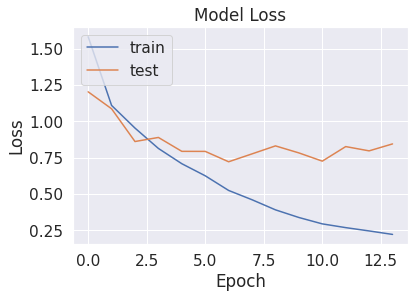
\includegraphics[width=0.8\textwidth]{images/q1/pb/loss}
	\caption{Validation and Training Loss}
	\label{fig:q1pbloss}
\end{figure}

The final output shows an average precision and recall of 83\% and 84\%
respectively, with the highest
values attributed to the ``Parachute'' class, and the lowest values attributed
to the ``English Springer'' class.

\begin{figure}[H]
	\centering
	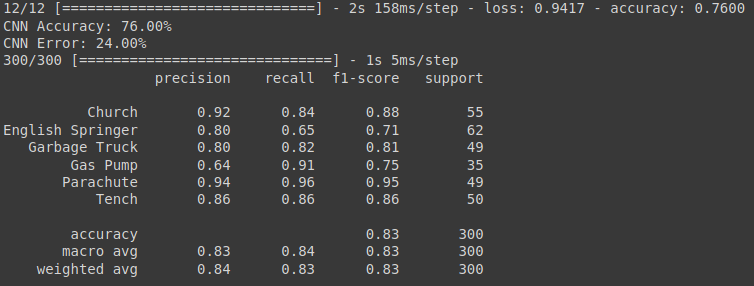
\includegraphics[width=0.8\textwidth]{images/q1/pb/results}
	\caption{Model Testing Results}
	\label{fig:q1pbResults}
\end{figure}

The confusion matrix shows the number of correctly identified samples during
testing. It is clear that the class with the highest precision and recall is
``Parachute'', labelled as ``4'' within the matrix.

\begin{figure}[H]
	\centering
	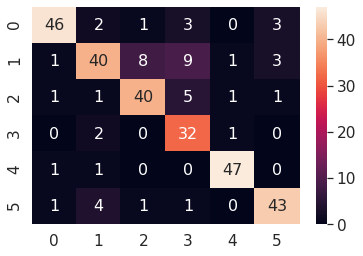
\includegraphics[width=0.8\textwidth]{images/q1/pb/matrix}
	\caption{Confusion Matrix}
	\label{fig:q1pbMatrix}
\end{figure}

Using early stopping, the model ran for a total of 14 epochs. The training time
for the model was 493.8769 seconds, which gives an emission output of 2.058lbs
CO2 equivalent emissions. This value is much higher than the value in Part a.
